\subsection{Idea general del problema}
Se ha decidido conectar telegráficamente todas las estaciones de un sistema férreo que recorre el país en abanico con origen en la capital (el kilómetro 0). Se nos ofrece cierta cantidad de kilometros de cable para conectar la ciudades de cada ramal. Al ser escaso el presupuesto, se busca lograr conectar la mayor cantidad de ciudades con los metros asignados, sin hacer cortes en el cable. \\

Se nos propone resolver cuántas ciudades se pueden conectar para cada ramal, con una complejidad de O(n), siendo n la cantidad de estaciones en cada ramal.\\

Para ello se nos brinda un archivo de entrada, el cual tiene para cada ramal dos líneas: la primera contiene un entero con los kilómetros de cable dedicados al ramal y la segunda los kilometrajes de las estaciones en el ramal sin considerar el 0. Luego de ejecutar nuestro algoritmo, la salida del mismo debe contener, para cada ramal de la entrada, una línea con la cantidad de ciudades conectables encontradas.\\

Un ejemplo de archivo de entrada puede ser, (extracto del archivo Tp1Ej1.in):\\
6 \\
6 8 12 15 \\
35 \\
8 14 20 40 45 54 60 67 74 89 99 \\
100 \\
35 87 141 163 183 252 288 314 356 387 \\
90 \\
6 8 16 19 28 32 37 45 52 60 69 78 82 \\

El mismo indica, en su primer línea que para el ramal 1 tenemos 6km de cable, y en su segunda línea que dicho ramal contiene (además de la capital, implícita, en el kilómetro 0) una estación en el kilómetro 6, otra en el 8, otra en el 12 y la última en el kilómetro 15. Luego para el ramal 2, tenemos 35 kilómetros de cable, y estaciones en los kilómetros: 8 14 20 40 45 54 60 67 74 89 y 99. Así sucesivamente para el resto de los ramales.\\

El archivo de salida luego de ejecutarse nuestro algoritmo deberá ser de la siguiente pinta, (extracto del archivo Tp1Ej1.out):\\
3 \\
6 \\
4 \\
14 \\

Este último archivo indica la cantidad de ciudades que se pueden conectar para cada ramal. En el caso del ramal 1, para el cual se tienen 6km de cable disponibles, y contiene ciudades en los kilómetros: 0 6 8 12 15 vemos que la solución debería ser que se pueden conectar como máximo 3 ciudades, a continuación explicaremos cómo se deduce esto.\\

Si conectamos la capital con la ciudad del kilómetro 6, al tener sólo 6km de cable, nuestra solución sería que pudimos conectar sólo 2 ciudades. Pero como debemos maximizar esta cantidad, podemos ver que si en vez de conectar a la capital con la primer estación del ramal, conectamos la ciudad del kilómetro 6, con su siguiente y con la del kilómetro 12, entonces como entre el kilómetro 6 y el 8 hay una diferencia de 2kms y entre el 8 y el 12 una diferencia de 4kms, vemos que la máxima cantidad de estaciones conectadas con 6km de cable para el ramal 1, es 3. La misma lógica se la aplica para los ramales restantes.\\


\subsection{Explicación y pseudocódigo}

int conectar(vector$<$int$>$ v , int longitud del cable) \{ \\
$~~~~~~~~~~~~$int resTemp $\leftarrow$ 1 \Ode{1}\\
$~~~~~~~~~~~~$int start $\leftarrow$ 0 \Ode{1}\\
$~~~~~~~~~~~~$int actual $\leftarrow$ 0 \Ode{1}\\
$~~~~~~~~~~~~$int aux $\leftarrow$ 0 \Ode{1}\\
$~~~~~~~~~~~~$\textbf{mientras} (la longitud del cable sea $>$ 0 y v[actual] no sea el ultimo) \{ \\ \WhileOde{n} \\
$~~~~~~~~~~~~~~~$aux  $\leftarrow$ longitud del cable \Ode{1}\\
$~~~~~~~~~~~~~~~$longitud del cable - (elemento próximo - elemento actual).\Ode{1}\\
$~~~~~~~~~~~~~~~$\textbf{si} (la longitud del cable sigue $\geq$ 0) \{ \\ \IfOde{1}\\
$~~~~~~~~~~~~~~~~~~~~~~$incrementamos en 1 resTemp\Ode{1}\\
$~~~~~~~~~~~~~~~~~~~~~~$incrementamos en 1 actual\Ode{1}\\
$~~~~~~~~~~~~~~~$\} \\ 
$~~~~~~~~~~~~$\} \\ 
$~~~~~~~~~~~~$int conectadas $\leftarrow$ resTemp \Ode{1}\\
$~~~~~~~~~~~~$\textbf{si} (resTemp sigue valiendo 1)\{ \\ \IfOde{1}\\
$~~~~~~~~~~~~~~~$ seteamos resTemp $\leftarrow$ 0; porque no se conectó ninguna ciudad. \Ode{1}\\
$~~~~~~~~~~~~$\} \\ 
$~~~~~~~~~~~~$\textbf{si} (nos pasamos y la longitud del cable $<$ 0) \{ \\  \IfOde{1} \\
$~~~~~~~~~~~~~~~$volvemos al valor anterior: la longitud del cable $\leftarrow$ aux\Ode{1}\\
$~~~~~~~~~~~~$\} \\ 
$~~~~~~~~~~~~$\textbf{mientras} (el elemento actual no sea el último) \{  \\ \WhileOde{n} \\
$~~~~~~~~~~~~~~~$\textbf{si}(resTemp == 0) \{ \\ \IfOde{1} \\
$~~~~~~~~~~~~~~~~~~~~$conectadas  $\leftarrow$ 0; \Ode{1}\\
$~~~~~~~~~~~~~~~~~~~~$incrementamos start en 1;  \Ode{1}\\
$~~~~~~~~~~~~~~~~~~~~$incrementamos actual en 1;  \Ode{1}\\
$~~~~~~~~~~~~~~~$\} \textbf{si no} \{ \\
$~~~~~~~~~~~~~~~~~~~~$decrementamos conectadas en 1;\Ode{1}\\ 
$~~~~~~~~~~~~~~~~~~~~$a longitud del cable le sumamos (v[start+1]-v[start]);\Ode{1}\\
$~~~~~~~~~~~~~~~~~~~~$incrementamos start en 1;  \Ode{1}\\
$~~~~~~~~~~~~~~~$\} \\
$~~~~~~~~~~~~~~~$\textbf{mientras}(longitud del cable $\geq$ 0 y v[actual] no es el último) \{ \\ \WhileOde{longitud del cable} \\
$~~~~~~~~~~~~~~~~~~~~$aux $\leftarrow$ longitud del cable \Ode{1}\\
$~~~~~~~~~~~~~~~~~~~~$a longitud del cable  le restamos (v[actual+1]- v[actual]); \Ode{1}\\
$~~~~~~~~~~~~~~~~~~~~$\textbf{si} (longitud del cable $\geq$ 0) \{ \\ \IfOde{1}\\
$~~~~~~~~~~~~~~~~~~~~~~~~~~$incrementamos conectadas en 1  \Ode{1}\\
$~~~~~~~~~~~~~~~~~~~~~~~~~~$incrementamos actual en 1  \Ode{1}\\
$~~~~~~~~~~~~~~~~~~~~$\} \\
$~~~~~~~~~~~~~~~~$\} \\
$~~~~~~~~~~~~~~~~$\textbf{si} (longitud del cable $<$ 0 ) \{ \\ \IfOde{1}\\
$~~~~~~~~~~~~~~~~~~~~$longitud del cable $\leftarrow$aux\Ode{1}\\
$~~~~~~~~~~~~~~~~$\} \\
$~~~~~~~~~~~~~~~~$\textbf{si} (conectadas $>$ resTemp) \{ \\ \IfOde{1}\\
$~~~~~~~~~~~~~~~~~~~~$resTemp $\leftarrow$ conectadas\Ode{1}\\
$~~~~~~~~~~~~~~~~$\} \\
$~~~~~~~~~~~~$\} \\
$~~~~~~~~~~~~$\textbf{si} (resTemp es 1) \{ \\ \IfOde{1}\\
$~~~~~~~~~~~~~~~~~~~~$resTemp $\leftarrow$ 2;\Ode{1}\\
$~~~~~~~~~~~~$\} \\
$~~~~~~~~~~~~$devolvemos resTemp \Ode{1} \\
\}\\

\subsection{Deducción de la cota de complejidad temporal}


Dedujimos que el algoritmo indica cuantas ciudades se pueden conectar para cada ramal en O(n), siendo n la cantidad de estaciones en cada ramal. Nuestro algoritmo cuenta con dos while independientes: El primer while sirve para ver hasta donde llega el cable empezando por la ciudad del kilómetro 0. Se ejecuta como mucho n veces, en ese caso (que es cuando el cable es lo suficientemente largo como para conectar todas las ciudades), el segundo while no se ejecutara pues ya se llegó al final, en caso contrario, si no se alcanza la última ciudad en el primer ciclo, este segundo ciclo desconecta la primer ciudad y se fija hasta que ciudad se llega ahora, sumándole al cable la distancia correspondiente entre la primer ciudad conectada y la segunda. Se ejecuta como mucho n veces (ese sería el peor caso, que ocurre cuando se da un cable muy corto y en cada iteración se avanza una o ninguna ciudad) dentro de él hay otro while que se ejecuta mientras que la longitud del cable sea positiva y hace lo dicho anteriormente, con la nueva longitud del cable se fija hasta que ciudad se llegaría, por ende mientras más largo el cable más ciudades se conectan y se van reduciendo las iteraciones del segundo while, ya que éste se ejecutaba hasta que se llegue a la última ciudad.\\

Usamos las funciones $>$, $<$, $\geq$, $+$, $-$, $==$, de complejidad constante al igual que las asignaciones. También sabemos por la documentación de C++, que el $operator[]$ del vector es de complejidad O(1) y la función del vector $.back()$ es también O(1).\\

Vamos a mostrar la implementación de un test generado sin ninguna intencionalidad, pero antes explicaremos detalladamente como fue creado. \\

Implementamos una función que genera números random para el archivo que le vamos a pasar por entrada a nuestro algoritmo con los siguientes criterios:
\begin{itemize}
\item Elegimos en este ejemplo que el primer ramal iba a contar con una estación, el segundo con 101, el tercero con 201 y asi sumando de a 100.
\item Para el valor de la longitud de cable disponible de cada ramal, decidimos que sea un número random entre 1 y la cantidad de estaciones de cada ramal.
\item Para los kilometrajes de las estaciones tuvimos en cuenta, que estos debían estar ordenados de menor a mayor, sin contener el kilómetro 0. Para definir esto hacemos algo de la pinta:

ciudad = ciudad + (random.randrange(i+1)+1)

random.randrange(i+1) da un número random entre 0 e $i+1$, como inicialmente $i$ es 0 tuvimos que sumarle 1. A su vez a esto lo incrementamos en 1 porque un número random entre 0 e $i+1$ puede llegar a darnos 0, y no queremos que esto pase, ya que el kilómetro 0 no debe figurar en el archivo de entrada.

Por otro lado, al hacer $``$ciudad = ciudad + ...$"$ nos aseguramos que los kilometrajes esten en orden creciente.

\end{itemize}

Podemos ver el código de este test implementado en python acá:

--------------------------------------------------------------------------------\\
$~~~~~~$file = open('ejemploConNumerosRandom.in', 'w+')\\
$~~~~~~$file2 = open('ejemploTamCiudades.txt', 'w+')\\
$~~~~~~$for x in xrange(1,10000, 100):\\
$~~~~~~~~~~~~$i = 0\\
$~~~~~~~~~~~~$ciudad = 0\\
$~~~~~~~~~~~~$file.write(str(random.randrange(x)) + ' \textbackslash n')\\
$~~~~~~~~~~~~$file2.write(str(x) + ' \textbackslash n')\\
$~~~~~~~~~~~~$while i $<$ x:\\
$~~~~~~~~~~~~~~~~~~~~~~~~$ciudad = ciudad + (random.randrange(i+1)+1)\\
$~~~~~~~~~~~~~~~~~~~~~~~~$file.write(str(ciudad) + ' ')\\
$~~~~~~~~~~~~~~~~~~~~~~~~$i = i + 1\\
$~~~~~~~~~~~~$file.write(' \textbackslash n')\\
$~~~~~~$file2.close()\\

--------------------------------------------------------------------------------\\

Una vez que generamos el archivo del input con dicho test, ejecutamos nuestro algoritmo obteniendo el archivo de salida con la cantidad de ciudades conectadas para cada ramal, e imprimimos por pantalla el tiempo promedio en milisegundos que tardó nuestro algoritmo en calcular la máxima cantidad de estaciones conectadas de cada ramal. ¿Por qué el tiempo promedio? Bueno, al ejecutarlo un par de veces nos dimos cuenta que se obtenían valores parecidos pero no idénticos, entonces decidimos correr el algoritmo una cierta cantidad de iteraciones (en este caso 100), e ir acumulando los tiempos para luego dividir este acumulador por 100 y así obtener un valor promedio de los tiempos en los que se tarda en resolver el problema para cada ramal. \\

Con estos tiempos creamos el gráfico de la figura \ref{ej1-tiempo-vs-cant-ciudades-random} que mostramos a continuación, en el que hacemos una comparación con la gráfica de O(n) y observamos como nuestro algoritmo cumple dicha complejidad.


\begin{figure}[H]
\begin{center}

\minipage{0.8\textwidth}
  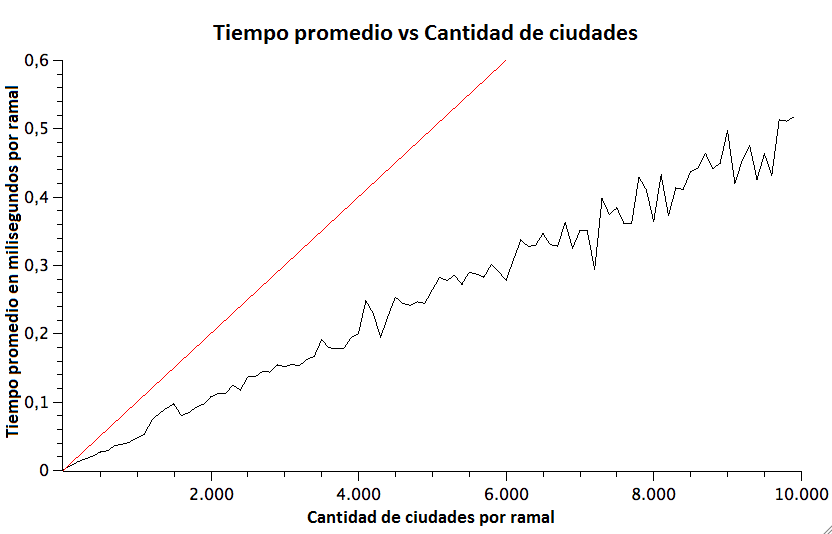
\includegraphics[width=\linewidth]{../graficos/ej1/1erEjTiempoPromedioVsO(n).png}
  \caption{{\small Comparación con O(n). Dado un archivo de entrada con longitud de cable y kilometrajes de estaciones random.}} \label{ej1-tiempo-vs-cant-ciudades-random}
\endminipage

\end{center}
\end{figure}
\subsection{Demostración formal}
\subsection{Experimentaciones}